%%%%%%%%%%%%%%%%%%%%%%%%%%%%%%%%%%%%%%%%%%%%%%%%%%%%%%%%%%%%%%%%%%%%%%%%%%%%%%%%%%
\begin{frame}[fragile]\frametitle{}
\begin{center}
{\Large ``Houston, we have a problem!!''}
\end{center}
\end{frame}

%%%%%%%%%%%%%%%%%%%%%%%%%%%%%%%%%%%%%%%%%%%%%%%%%%%%%%%%%%%
\begin{frame}[fragile]\frametitle{The Problem}
Every company is claiming to be working in AI-ML
\begin{itemize}
\item Is it really so?
\item What exactly is AI (ML)?
\item What is not AI?
\end{itemize}
Or is it just a plain BIG hype?
\end{frame}


%%%%%%%%%%%%%%%%%%%%%%%%%%%%%%%%%%%%%%%%%%%%%%%%%%%%%%%%%%%
\begin{frame}[fragile]\frametitle{Technology Phases}
\begin{center}
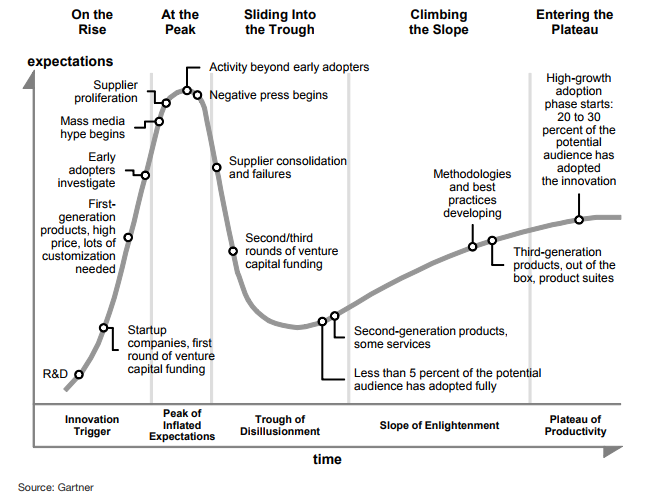
\includegraphics[width=0.8\linewidth,keepaspectratio]{gartner1old}
\end{center}
{\tiny (Ref: Understanding Gartner's Hype Cycles - Jackie Fenn, Mark Raskino, Betsy Burton )}
\end{frame}

%%%%%%%%%%%%%%%%%%%%%%%%%%%%%%%%%%%%%%%%%%%%%%%%%%%%%%%%%%%
\begin{frame}[fragile]\frametitle{2017 Hype Cycle}
\begin{center}
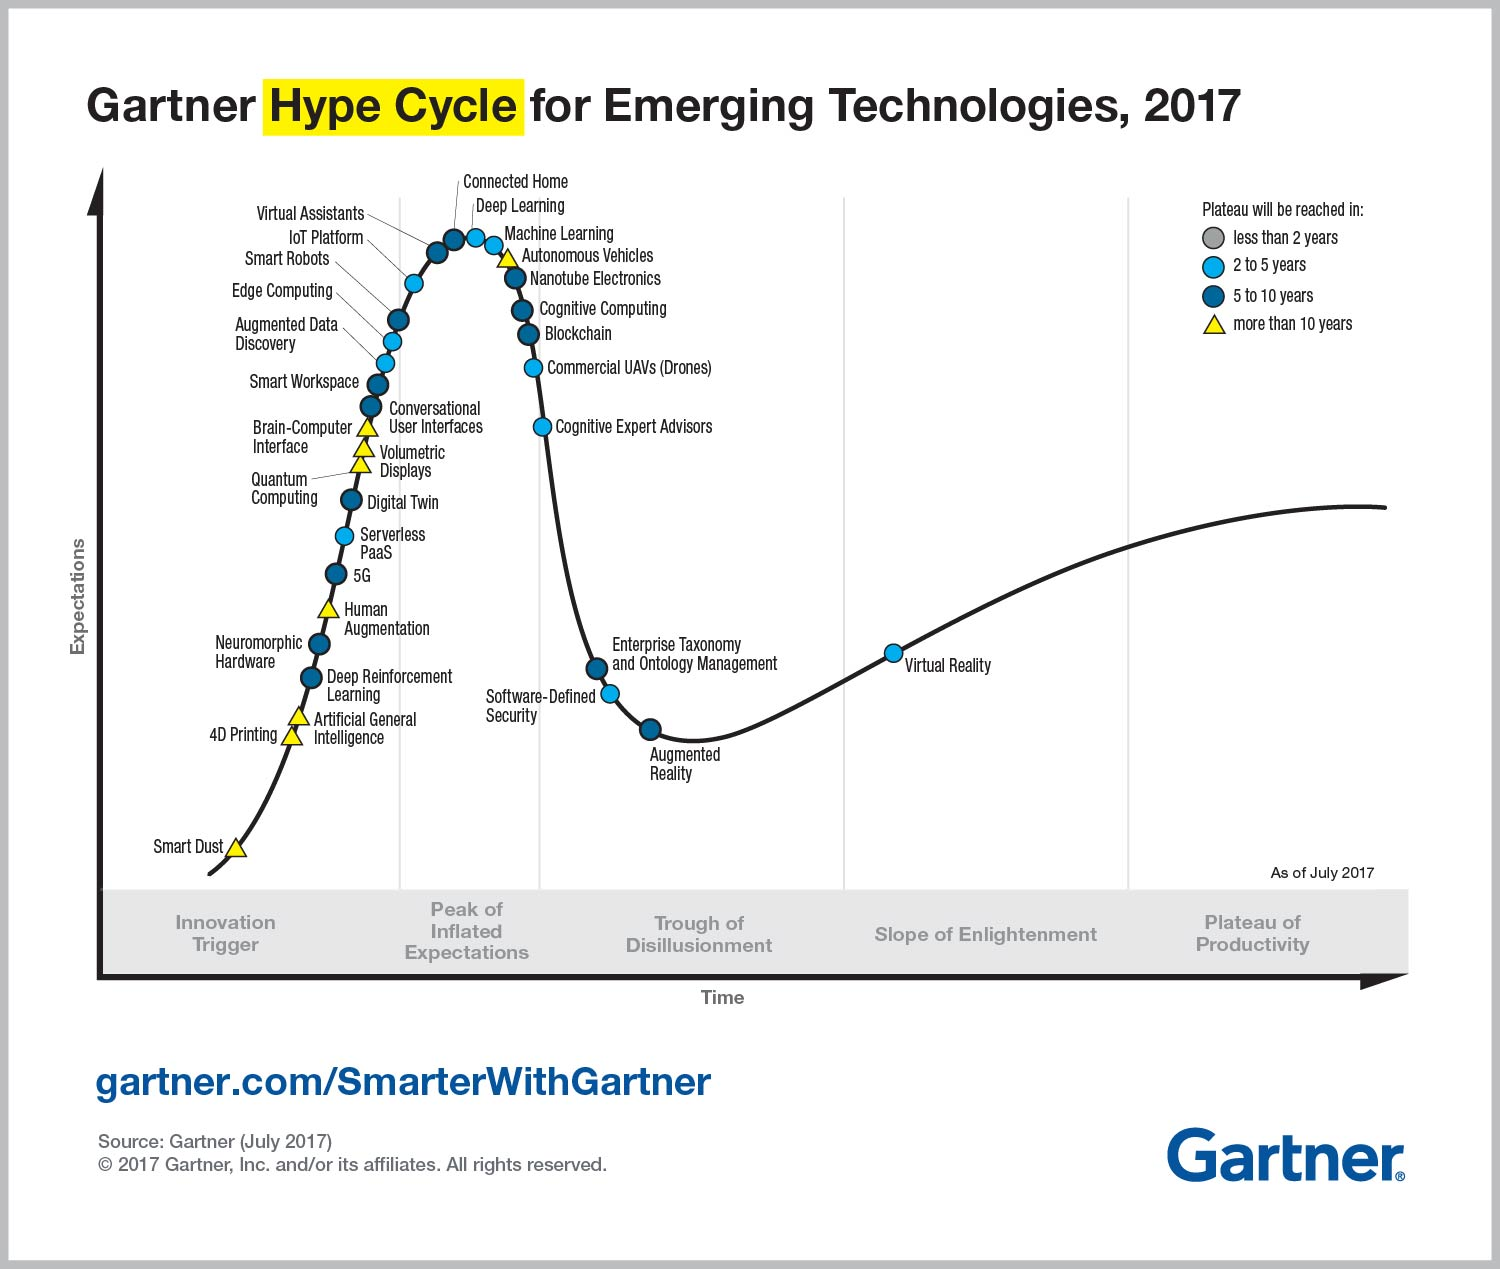
\includegraphics[width=0.8\linewidth,keepaspectratio]{gartner3_2017}
\end{center}
{\tiny (Ref: Understanding Gartner's Hype Cycles - Jackie Fenn, Mark Raskino, Betsy Burton )}
\end{frame}


%%%%%%%%%%%%%%%%%%%%%%%%%%%%%%%%%%%%%%%%%%%%%%%%%%%%%%%%%%%
\begin{frame}[fragile]\frametitle{The Peak}
\begin{itemize}
\item ``Machine Learning'', ``Deep Learning'' at the Peak
\item May take 2 to 5 years to mature well
\item If they survive disillusionment, then can be long term players
\end{itemize}
\end{frame}


% %%%%%%%%%%%%%%%%%%%%%%%%%%%%%%%%%%%%%%%%%%%%%%%%%%%%%%%%%%%
% \begin{frame}[fragile]\frametitle{What are the signs of being at the peak?}
% \begin{itemize}
% \item Featured on the front cover of every business magazine.
% \item Marketplace is flooded with offerings.
% \item  The technology is viewed as a panacea, without any regard to its
% suitability.
% \item Peer pressure on companies to adopt, without understanding challenges and risks
% \end{itemize}
% {\tiny (Ref: Understanding Gartner's Hype Cycles - Jackie Fenn, Mark Raskino, Betsy Burton )}
% \end{frame}

% %%%%%%%%%%%%%%%%%%%%%%%%%%%%%%%%%%%%%%%%%%%%%%%%%%%%%%%%%%%
% \begin{frame}[fragile]\frametitle{Bosses}
% \begin{center}
% \includegraphics[width=\linewidth,keepaspectratio]{dilbert2}
% \end{center}
% {\tiny (Ref: Dilbert )}
% \end{frame}

% %%%%%%%%%%%%%%%%%%%%%%%%%%%%%%%%%%%%%%%%%%%%%%%%%%%%%%%%%%%
% \begin{frame}[fragile]\frametitle{What do we do at such times?}
% \begin{itemize}
% \item Wait till everything plays out?
% \item Or get on the bandwagon, test the waters?
% \item Choice can be anything, but better to make an informed decision.
% \end{itemize}
% \end{frame}

% %%%%%%%%%%%%%%%%%%%%%%%%%%%%%%%%%%%%%%%%%%%%%%%%%%%%%%%%%%%
% \begin{frame}[fragile]\frametitle{What is so different?}
% \begin{itemize}
% %\item Amongst all this hype there one natural instinct
% %\item ``Research'', Understanding whats going on
% \item Just another set of problem solving techniques.
% \item Using the knowledge to solve problems, 
% \item either in better manner
% \item or tackle completely unsolvable problems 
% \end{itemize}
% \end{frame}

%%%%%%%%%%%%%%%%%%%%%%%%%%%%%%%%%%%%%%%%%%%%%%%%%%%%%%%%%%%%%%%%%%%%%%%%%%%%%%%%%%
\begin{frame}[fragile]\frametitle{}
\begin{center}
{\Large What is the Core Idea?}
\end{center}
\end{frame}

%%%%%%%%%%%%%%%%%%%%%%%%%%%%%%%%%%%%%%%%%%%%%%%%%%%%%%%%%%%%%%%%%%%%%%%%%%%%%%%%%%
\begin{frame}[fragile]\frametitle{What's the core idea?'}
\begin{itemize}
\item behind problem solving?
\item behind writing software algorithms?
\item solving research problems?
\end{itemize}
\end{frame}

%%%%%%%%%%%%%%%%%%%%%%%%%%%%%%%%%%%%%%%%%%%%%%%%%%%%%%%%%%%
\begin{frame}[fragile]\frametitle{Desire}
\begin{itemize}
\item To find a ``function''
\item To find a relation
\item To find a transformation
\item To build a model
\item From given inputs to desired outputs.
\end{itemize}
That's it.
\end{frame}

%%%%%%%%%%%%%%%%%%%%%%%%%%%%%%%%%%%%%%%%%%%%%%%%%%%%%%%%%%%
\begin{frame}[fragile]\frametitle{Functions}
\begin{itemize}
\item Some functions are straight forward
\item {\em ``In summer, ice-cream sale goes up''}
\item Cause and effect
\item Relation (function, Mathematical model) is found out
\item Here, simple rule based programming suffices
\end{itemize}
\end{frame}

%%%%%%%%%%%%%%%%%%%%%%%%%%%%%%%%%%%%%%%%%%%%%%%%%%%%%%%%%%%
\begin{frame}[fragile]\frametitle{Functions}
\begin{itemize}
\item But some functions are complex
\item {\em ``More you put efforts, your business flourishes.''}
\item Cause and effect again, but the relation is far to complex
\item Too many variables
\item Here, simple rule based programming not humanly possible.
\item Lots of research needed to come up with equations.
\end{itemize}
\end{frame}

%%%%%%%%%%%%%%%%%%%%%%%%%%%%%%%%%%%%%%%%%%%%%%%%%%%%%%%%%%%
\begin{frame}[fragile]\frametitle{Functions}
\begin{itemize}
\item $E = mc^2$
\item What's this? a function?
\item Input variable(s)?
\item Output variable(s)?
\item Parameters?
\item How's the relation? linear?
\end{itemize}
\end{frame}

%%%%%%%%%%%%%%%%%%%%%%%%%%%%%%%%%%%%%%%%%%%%%%%%%%%%%%%%%%%
\begin{frame}[fragile]\frametitle{Controversial Example}
\begin{itemize}
\item Even astrology is a model, based on the past cases.
\item Could claim imperical evidence. 
\item Given this planetary position, it predicts.
\item Represented by ``Horoscope''
\item Got weights for each planets (real or ficticous)
\item Reliable??
\end{itemize}
\end{frame}


%%%%%%%%%%%%%%%%%%%%%%%%%%%%%%%%%%%%%%%%%%%%%%%%%%%%%%%%%%%
\begin{frame}[fragile]\frametitle{Functions}
\begin{itemize}
\item But most real-life functions are not deterministic
\item Some are probabilistic, some non-linear.
\item {\em ``Detecting if the tumor is benign or malignant''}
\item {\em ``At any state in the game of chess, whats the next move?''}
\end{itemize}
\end{frame}

%%%%%%%%%%%%%%%%%%%%%%%%%%%%%%%%%%%%%%%%%%%%%%%%%%%%%%%%%%%
\begin{frame}[fragile]\frametitle{Chess: next move?}
\begin{itemize}
\item Needs extreme expertise
\item Needs ``intelligence''
\item How do you get that?
\begin{itemize}
\item Built by lots of training.
\item By studying lots of past games.
\end{itemize}
\item This is how Humans build intelligence
\end{itemize}
\end{frame}

%%%%%%%%%%%%%%%%%%%%%%%%%%%%%%%%%%%%%%%%%%%%%%%%%%%%%%%%%%%
\begin{frame}[fragile]\frametitle{Intelligence}
\begin{itemize}
\item Can machine (software/program) also do the same?
\item Can it play chess?
\item Can it build intelligence?
\item By looking at past experiences (data), 
\item Training Data: games played, moves used, etc.
\end{itemize}
Yes, it can!! Thats Artificial Intelligence.
\end{frame}

%%%%%%%%%%%%%%%%%%%%%%%%%%%%%%%%%%%%%%%%%%%%%%%%%%%%%%%%%%%%%%%%%%%%%%%%%%%%%%%%%%
\begin{frame}[fragile]\frametitle{}
\begin{center}
{\Large What is AI?}
\end{center}
\end{frame}



%%%%%%%%%%%%%%%%%%%%%%%%%%%%%%%%%%%%%%%%%%%%%%%%%%%%%%%%%%%
\begin{frame}[fragile]\frametitle{ What is Artificial Intelligence (AI)?}
My definition:


``If machines (or computer programs) start doing some/all of these ``intelligent'' tasks, then that's Artificial Intelligence''

\end{frame}

%%%%%%%%%%%%%%%%%%%%%%%%%%%%%%%%%%%%%%%%%%%%%%%%%%%%%%%%%%%
\begin{frame}[fragile]\frametitle{ Intelligence: the differentiation}
\begin{itemize}
\item Ability to think various domains
\item Ability produce something new
\item Ability to detect the unseen
\item Ability to enhance knowledge (rules, patterns)
\end{itemize}
All these, AI has started doing. The AI era has arrived!!
\end{frame}

%%%%%%%%%%%%%%%%%%%%%%%%%%%%%%%%%%%%%%%%%%%%%%%%%%%%%%%%%%%
\begin{frame}[fragile]\frametitle{ What is Artificial Intelligence (AI)?}
 As Bernard Marr comments in Forbes, there is a need to distinguish between ``the ability to replicate or imitate human thought'' that has driven much AI to more recent models which ``use human reasoning as a model but not an end goal''.

\end{frame}

% %%%%%%%%%%%%%%%%%%%%%%%%%%%%%%%%%%%%%%%%%%%%%%%%%%%%%%%%%%%
% \begin{frame}[fragile]\frametitle{ What is Artificial Intelligence (AI)?}
% \begin{center}
% \includegraphics[width=0.6\linewidth,keepaspectratio]{ai64}
% \end{center}

% {\tiny (Ref:  Here's the 8 types of Artificial Intelligence, and what you should know about them - Jen Hyatt)}
% \end{frame}

%%%%%%%%%%%%%%%%%%%%%%%%%%%%%%%%%%%%%%%%%%%%%%%%%%%%%%%%%%%
\begin{frame}[fragile]\frametitle{AI era}
\begin{itemize}
\item Coming of the fourth industrial revolution
\item More important than Electricity - Google
\end{itemize}

``AI happening ten times faster and at 300 times the scale or at roughly 3,000 times the impact of the Industrial Revolution'' - McKinsey

{\tiny (Ref: https://www.mckinsey.com/~/media/McKinsey/Business Functions/Strategy and Corporate Finance/Our Insights/Strategy and corporate finance special collection/Final PDFs/McKinsey-Special-Collections\_Trends-and-global-forces.ashx)}
\end{frame}

% %%%%%%%%%%%%%%%%%%%%%%%%%%%%%%%%%%%%%%%%%%%%%%%%%%%%%%%%%%%
%\begin{frame}[fragile]\frametitle{Intelligence}
% \begin{itemize}
%\item Some models give insight of what happened, using past data..mostly say BI, in commercial context
%\item Some models give prediction of what MAY happen in future, that's Machine learning (part of AI)
% \end{itemize}
% \end{frame}


%%%%%%%%%%%%%%%%%%%%%%%%%%%%%%%%%%%%%%%%%%%%%%%%%%%%%%%%%%%
\begin{frame}[fragile]\frametitle{Everyday usage}
Artificial intelligence seems to have become ubiquitous.
\begin{itemize}
\item Replying to our emails on Gmail
\item Learning how to drive our cars,
\item Sorting our holiday photos.
\item etc.
\end{itemize}
Too good to be true, isn't it, sort of Magical !!
\end{frame}

%%%%%%%%%%%%%%%%%%%%%%%%%%%%%%%%%%%%%%%%%%%%%%%%%%%%%%%%%%%
\begin{frame}[fragile]\frametitle{But then \ldots}
\begin{itemize}
\item When its too good, you start suspecting
\item Is it for real!!
\item How can such thing happen?
\item How far will it go?
\end{itemize}
The next thing you know, people are worrying about exactly how and when AI is going to doom humanity.
\end{frame}

%%%%%%%%%%%%%%%%%%%%%%%%%%%%%%%%%%%%%%%%%%%%%%%%%%%%%%%%%%%%%%%%%%%%%%%%%%%%%%%%%%
\begin{frame}[fragile]\frametitle{}
\begin{center}
{\Large Is AI new?}
\end{center}
\end{frame}



%%%%%%%%%%%%%%%%%%%%%%%%%%%%%%%%%%%%%%%%%%%%%%%%%%%%%%%%%%%
\begin{frame}[fragile]\frametitle{Is AI new? A little history}
\begin{center}
\includegraphics[width=0.8\linewidth,keepaspectratio]{aipaper}
\end{center}
{\tiny (Ref:  John McCarthy, Marvin L. Minsky, Nathaniel Rochester, and Claude E. Shannon (1955))}
\end{frame}

%%%%%%%%%%%%%%%%%%%%%%%%%%%%%%%%%%%%%%%%%%%%%%%%%%%%%%%%%%%
\begin{frame}[fragile]\frametitle{Is AI new? A little history}
\begin{center}
\includegraphics[width=0.8\linewidth,keepaspectratio]{aihist}
\end{center}
{\tiny (Ref:  What Exactly is Artificial Intelligence and Why is it Driving me Crazy - William Vorhies)}
\end{frame}

%%%%%%%%%%%%%%%%%%%%%%%%%%%%%%%%%%%%%%%%%%%%%%%%%%%%%%%%%%%
\begin{frame}[fragile]\frametitle{Turing Test}
\begin{center}
\includegraphics[width=0.6\linewidth,keepaspectratio]{Turing}
\end{center}
Simplistically: If you cannot decide if you are talking to a human or a machine then AI has arrived.
{\tiny (Ref:  What is Artificial Intelligence | Artificial Intelligence Tutorial For Beginners | Edureka)}
\end{frame}


%%%%%%%%%%%%%%%%%%%%%%%%%%%%%%%%%%%%%%%%%%%%%%%%%%%%%%%%%%%%
%\begin{frame}[fragile]\frametitle{A little history (cont'd)}
%7 main key requirements of AI: 
%\begin{itemize}
%\item  Automatic computer
%\item  Language understanding
%\item  Usage of neuron nets
%\item  Computational efficiency
%\item  Self-improvement
%\item  Abstractions
%\item  Creativity 
%\end{itemize}
%{\tiny (Ref:  John McCarthy, Marvin L. Minsky, Nathaniel Rochester, and Claude E. Shannon (1955))}
%\end{frame}



% %%%%%%%%%%%%%%%%%%%%%%%%%%%%%%%%%%%%%%%%%%%%%%%%%%%%%%%%%%%
% \begin{frame}[fragile]\frametitle{Types of Artificial Intelligence}
% \begin{itemize}
% \item  ``Strong'' or ``General'' Artificial Intelligence
% \item  ``Weak'' or ``Specific'' Artificial Intelligence
% \end{itemize}
% \end{frame}

% %%%%%%%%%%%%%%%%%%%%%%%%%%%%%%%%%%%%%%%%%%%%%%%%%%%%%%%%%%%
% \begin{frame}[fragile]\frametitle{Strong Artificial Intelligence}
% \begin{itemize}
% \item   Computers thinking at a level that meets or surpasses people
% \item   Computers engaging in abstract reasoning \& thinking
% \item   This is not what we have today
% \item   There is no evidence that we are close to Strong AI
% \end{itemize}
% \end{frame}

% %%%%%%%%%%%%%%%%%%%%%%%%%%%%%%%%%%%%%%%%%%%%%%%%%%%%%%%%%%%
% \begin{frame}[fragile]\frametitle{Weak Artificial Intelligence}
% \begin{itemize}
% \item   Computers solve problems by detecting useful patterns
% \item   Pattern-based AI is an Extremely powerful tool 
% \item   Has been used to automate many processes today
% \item   Driving, language translation
% \item   This is the dominant mode of AI today
% \end{itemize}
% \end{frame}


%%%%%%%%%%%%%%%%%%%%%%%%%%%%%%%%%%%%%%%%%%%%%%%%%%%%%%%%%%%
\begin{frame}[fragile]\frametitle{Major AI Approaches}
\begin{itemize}
\item  Logic and Rules-Based Approach
\item  Machine Learning (Pattern-Based Approach)
\end{itemize}
\end{frame}

%%%%%%%%%%%%%%%%%%%%%%%%%%%%%%%%%%%%%%%%%%%%%%%%%%%%%%%%%%%
\begin{frame}[fragile]\frametitle{Logic and Rules-Based Approach}
\begin{itemize}
\item  Representing processes or systems using logical rules
\item Top-down rules are created for computer
\item Computers reason about those rules
\item Can be used to automate processes
\end{itemize}
\end{frame}

%%%%%%%%%%%%%%%%%%%%%%%%%%%%%%%%%%%%%%%%%%%%%%%%%%%%%%%%%%%
\begin{frame}[fragile]\frametitle{Logic and Rules-Based Approach}
Example :  Expert Systems, Turbotax/Tally
\begin{itemize}
\item  Personal income tax laws 
\item  Represented as logical computer rules
\item  Software computes tax liability
\end{itemize}
\end{frame}

%%%%%%%%%%%%%%%%%%%%%%%%%%%%%%%%%%%%%%%%%%%%%%%%%%%%%%%%%%%
\begin{frame}[fragile]\frametitle{Machine Learning (Pattern based)}
\begin{itemize}
\item  Algorithms find patterns in data and infer rules on their own
\item   ``Learn'' from data and improve over time
\item  These patterns can be used for automation or prediction
\item  ML is the dominant mode of AI today
\item Deep Learning is one set of methods within ML
\end{itemize}
\end{frame}

%%%%%%%%%%%%%%%%%%%%%%%%%%%%%%%%%%%%%%%%%%%%%%%%%%%%%%%%%%%
\begin{frame}[fragile]\frametitle{Machine Learning (Pattern based)}
\begin{itemize}
\item Learning from Data
\item Pattern Detection
\item Self-Programming/Automation
\end{itemize}
\end{frame}

%
%
%%%%%%%%%%%%%%%%%%%%%%%%%%%%%%%%%%%%%%%%%%%%%%%%%%%%%%%%%%%%
%\begin{frame}[fragile]\frametitle{Example: Email Spam Filter}
%\begin{center}
%\includegraphics[width=0.8\linewidth,keepaspectratio]{ai4}
%\end{center}
%{\tiny (Ref: ``Artificial Intelligence Overview'' - Harry Surden )}
%\end{frame}
%
%
%%%%%%%%%%%%%%%%%%%%%%%%%%%%%%%%%%%%%%%%%%%%%%%%%%%%%%%%%%%%
%\begin{frame}[fragile]\frametitle{Example: Email Spam Filter}
%\begin{center}
%\includegraphics[width=0.8\linewidth,keepaspectratio]{ai5}
%\end{center}
%{\tiny (Ref: ``Artificial Intelligence Overview'' - Harry Surden )}
%\end{frame}
%
%
%%%%%%%%%%%%%%%%%%%%%%%%%%%%%%%%%%%%%%%%%%%%%%%%%%%%%%%%%%%%
%\begin{frame}[fragile]\frametitle{Intelligence mimicked}
%\begin{itemize}
%\item For some (not all) complex tasks requiring intelligence
%\item Can get ``intelligent'' automated results without intelligence
%\item By finding suitable proxies or patterns
%\end{itemize}
%\end{frame}
%
%%%%%%%%%%%%%%%%%%%%%%%%%%%%%%%%%%%%%%%%%%%%%%%%%%%%%%%%%%%%
%\begin{frame}[fragile]\frametitle{Proxies}
%New: Statistical Machine Translation
%\begin{itemize}
%\item People use advanced cognitive skills to translate
%\item Google finds statistical correlations by analyzing previously translated documents
%\item Produces automated translations using statistical likelihood as a ``proxy'' for underlying meaning
%\end{itemize}
%\end{frame}

%%%%%%%%%%%%%%%%%%%%%%%%%%%%%%%%%%%%%%%%%%%%%%%%%%%%%%%%%%%
\begin{frame}[fragile]\frametitle{Relationship between AI, ML, DL}
\begin{center}
\includegraphics[width=\linewidth,keepaspectratio]{ai1}
\end{center}
{\tiny (Ref: https://blogs.nvidia.com/blog/2016/07/29/whats-difference-artificial-intelligence-machine-learning-deep-learning-ai/)}
\end{frame}

% %%%%%%%%%%%%%%%%%%%%%%%%%%%%%%%%%%%%%%%%%%%%%%%%%%%%%%%%%%%
% \begin{frame}[fragile]\frametitle{AI/ML/DL Example}
% \begin{center}
% \includegraphics[width=0.8\linewidth,keepaspectratio]{ml1}
% \end{center}

% {\tiny (Ref:  What is Artificial Intelligence | Artificial Intelligence Tutorial For Beginners | Edureka)}
% \end{frame}

% %%%%%%%%%%%%%%%%%%%%%%%%%%%%%%%%%%%%%%%%%%%%%%%%%%%%%%%%%%%
% \begin{frame}[fragile]\frametitle{AI/ML/DL Example}
% \begin{center}
% \includegraphics[width=0.8\linewidth,keepaspectratio]{ml2}
% \end{center}

% {\tiny (Ref:  What is Artificial Intelligence | Artificial Intelligence Tutorial For Beginners | Edureka)}
% \end{frame}


% %%%%%%%%%%%%%%%%%%%%%%%%%%%%%%%%%%%%%%%%%%%%%%%%%%%%%%%%%%%
% \begin{frame}[fragile]\frametitle{AI/ML/DL Example}
% \begin{center}
% \includegraphics[width=0.8\linewidth,keepaspectratio]{ml3}
% \end{center}

% {\tiny (Ref:  What is Artificial Intelligence | Artificial Intelligence Tutorial For Beginners | Edureka)}
% \end{frame}


% %%%%%%%%%%%%%%%%%%%%%%%%%%%%%%%%%%%%%%%%%%%%%%%%%%%%%%%%%%%
% \begin{frame}[fragile]\frametitle{Deep Learning}
% \begin{itemize}
% \item Uses Neural Networks.
% \item Networks comprised of Nodes (Data Structures in computer program)
% \item Mimic human brains neurons.
% \item Each node is like a function which accepts inputs, does processing and returns output
% \item With different structures of this network, various phenomenon can be modeled, mathematically
% \item Like $2x_1 + 3x_2$ can be modeled.
% \item Thus, many real life problems can be modeled and solved
% \end{itemize}
% \end{frame}

% %%%%%%%%%%%%%%%%%%%%%%%%%%%%%%%%%%%%%%%%%%%%%%%%%%%%%%%%%%%
% \begin{frame}[fragile]\frametitle{Deep Learning Network}
% \begin{center}
% \includegraphics[width=0.8\linewidth,keepaspectratio]{dl25}
% \end{center}

% {\tiny (Ref:  What is Artificial Intelligence | Artificial Intelligence Tutorial For Beginners | Edureka)}
% \end{frame}

% %%%%%%%%%%%%%%%%%%%%%%%%%%%%%%%%%%%%%%%%%%%%%%%%%%%%%%%%%%%%%%%%%%%%%%%%%%%%%%%%%%
% \begin{frame}[fragile]\frametitle{}
% \begin{center}
% {\Large AI Applications}
% \end{center}
% \end{frame}


% %%%%%%%%%%%%%%%%%%%%%%%%%%%%%%%%%%%%%%%%%%%%%%%%%%%%%%%%%%%
% \begin{frame}[fragile]\frametitle{AI/ML/DL Applications}
% \begin{center}
% \includegraphics[width=0.8\linewidth,keepaspectratio]{apps1}
% \end{center}

% {\tiny (Ref:  What is Artificial Intelligence | Artificial Intelligence Tutorial For Beginners | Edureka)}
% \end{frame}

% %%%%%%%%%%%%%%%%%%%%%%%%%%%%%%%%%%%%%%%%%%%%%%%%%%%%%%%%%%%
% \begin{frame}[fragile]\frametitle{AI/ML/DL Applications}
% \begin{center}
% \includegraphics[width=0.8\linewidth,keepaspectratio]{apps2}
% \end{center}

% {\tiny (Ref:  What is Artificial Intelligence | Artificial Intelligence Tutorial For Beginners | Edureka)}
% \end{frame}



% %%%%%%%%%%%%%%%%%%%%%%%%%%%%%%%%%%%%%%%%%%%%%%%%%%%%%%%%%%%
% \begin{frame}[fragile]\frametitle{When do we need AI?}
% For tasks that are beyond human capabilities 
% \begin{itemize}
% \item Analysis of large and complex data-sets 
% \item E.g. IBM Watson's Jeopardy-playing machine
% \end{itemize}
% \begin{center}
% \includegraphics[width=0.8\linewidth,keepaspectratio]{ai2}
% \end{center}
% {\tiny (Ref:  https://i.ytimg.com/vi/P18EdAKuC1U/maxresdefault.jpg )}
% \end{frame}

% %%%%%%%%%%%%%%%%%%%%%%%%%%%%%%%%%%%%%%%%%%%%%%%%%%%%%%%%%%%
% \begin{frame}[fragile]\frametitle{When do we need AI?}
 % Autopilot controls
% \begin{center}
% \includegraphics[width=0.8\linewidth,keepaspectratio]{ai3}
% \end{center}

% {\tiny (Ref:  https://media.newyorker.com/photos/59095c8a019dfc3494e9f7b9/ 16:9/w\_1200,h\_630,c\_limit/Hazards-of-Autopilot.jpg )}
% \end{frame}

% %%%%%%%%%%%%%%%%%%%%%%%%%%%%%%%%%%%%%%%%%%%%%%%%%%%%%%%%%%%
% \begin{frame}[fragile]\frametitle{Other Applications}
% %For tasks that are easily performed by humans but are complex for computer systems to emulate 
% \begin{itemize}
% \item Spam recognition in Emails
% \item Recommendation Systems
% \item Feelings Analysis, Sentiments
% \item Politics, Elections
% \item Identifying Billions of Dollars in Fraud
% \item Vision: Identify faces in a photograph, objects in a video
% \item Natural language: Translate a sentence from Hindi to English, question answering, etc. 
% \item Speech: Recognize spoken words, speaking sentences naturally 
% \item Game playing: Play games like chess 
% \item Robotics: Walking, jumping, displaying emotions, etc. 
% \item Driving a car, flying a plane, navigating a maze, etc.
% \end{itemize}
% \end{frame}

% %%%%%%%%%%%%%%%%%%%%%%%%%%%%%%%%%%%%%%%%%%%%%%%%%%%%%%%%%%%
% \begin{frame}[fragile]\frametitle{AI Systems}
% \begin{center}
% \includegraphics[width=0.8\linewidth,keepaspectratio]{aistack}
% \end{center}
% \end{frame}


%%%%%%%%%%%%%%%%%%%%%%%%%%%%%%%%%%%%%%%%%%%%%%%%%%%%%%%%%%%%%%%%%%%%%%%%%%%%%%%%%%
\begin{frame}[fragile]\frametitle{}
\begin{center}
{\Large Is AI a threat?}
\end{center}
\end{frame}

%%%%%%%%%%%%%%%%%%%%%%%%%%%%%%%%%%%%%%%%%%%%%%%%%%%%%%%%%%%
\begin{frame}[fragile]\frametitle{Is AI a threat?}
If you believe in what Elon Musk says, then YES.
\begin{center}
\includegraphics[width=0.8\linewidth,keepaspectratio]{nk}
\end{center}
{\tiny (Ref:  What is Artificial Intelligence | Artificial Intelligence Tutorial For Beginners | Edureka)}
\end{frame}

%%%%%%%%%%%%%%%%%%%%%%%%%%%%%%%%%%%%%%%%%%%%%%%%%%%%%%%%%%%
\begin{frame}[fragile]\frametitle{Is AI a threat?}
If you believe in these movies, then YES.
\begin{center}
\includegraphics[width=0.8\linewidth,keepaspectratio]{robots}
\end{center}
Well, AI based War robots are not impossible anymore.

{\tiny (Ref:  What is Artificial Intelligence | Artificial Intelligence Tutorial For Beginners | Edureka)}
\end{frame}


%%%%%%%%%%%%%%%%%%%%%%%%%%%%%%%%%%%%%%%%%%%%%%%%%%%%%%%%%%%
\begin{frame}[fragile]\frametitle{Fear: Are we being replaced?}
\begin{itemize}
\item Yes. in tasks that are repetitive
\item But not which require complex thinking and creativity
\end{itemize}
\end{frame}

%%%%%%%%%%%%%%%%%%%%%%%%%%%%%%%%%%%%%%%%%%%%%%%%%%%%%%%%%%%
\begin{frame}[fragile]\frametitle{Mostly}
Technology Enhancing (Not Replacing) Humans
\begin{center}
\includegraphics[width=0.8\linewidth,keepaspectratio]{ai6}
\end{center}
{\tiny (Ref: ``Artificial Intelligence Overview'' - Harry Surden )}
\end{frame}

%%%%%%%%%%%%%%%%%%%%%%%%%%%%%%%%%%%%%%%%%%%%%%%%%%%%%%%%%%%
\begin{frame}[fragile]\frametitle{Limits on Artificial Intelligence}
\begin{itemize}
\item  Many things still beyond the realm of AI
\item  No thinking computers
\item  No Abstract Reasoning
\item  Often AI systems Have Accuracy Limits
\item  Many things difficult to capture in data
\item  Sometimes Hard to interpret Systems
\end{itemize}
\end{frame}

%%%%%%%%%%%%%%%%%%%%%%%%%%%%%%%%%%%%%%%%%%%%%%%%%%%%%%%%%%%%%%%%%%%%%%%%%%%%%%%%%%%
%\begin{frame}[fragile]\frametitle{}
%\begin{center}
%{\Large Prediction time \ldots}
%\end{center}
%\end{frame}

% %%%%%%%%%%%%%%%%%%%%%%%%%%%%%%%%%%%%%%%%%%%%%%%%%%%%%%%%%%%
% \begin{frame}[fragile]\frametitle{Prediction time}
% 8 ways artificial intelligence is going to change the way you live, work and play in 2018
% % \end{frame}

% %%%%%%%%%%%%%%%%%%%%%%%%%%%%%%%%%%%%%%%%%%%%%%%%%%%%%%%%%%%
% \begin{frame}[fragile]\frametitle{Prediction time}
% 1. Everybody will have a virtual assistant, and they're going to be pretty smart ( My AI knows what I like!!!)
% \end{frame}

% %%%%%%%%%%%%%%%%%%%%%%%%%%%%%%%%%%%%%%%%%%%%%%%%%%%%%%%%%%%
% \begin{frame}[fragile]\frametitle{Prediction time}
% 2. All your voice-based gadgets will work together, from lamps, to TVs, to cars and beyond. 
% \end{frame}

% %%%%%%%%%%%%%%%%%%%%%%%%%%%%%%%%%%%%%%%%%%%%%%%%%%%%%%%%%%%
% \begin{frame}[fragile]\frametitle{Prediction time}
% 3. Facial recognition will be the new credit card, the new driver's license and the new bar-code.
% \end{frame}

% %%%%%%%%%%%%%%%%%%%%%%%%%%%%%%%%%%%%%%%%%%%%%%%%%%%%%%%%%%%
% \begin{frame}[fragile]\frametitle{Prediction time}
% 4. Artificial intelligence will generate media specific to your personal preferences
% \end{frame}

% %%%%%%%%%%%%%%%%%%%%%%%%%%%%%%%%%%%%%%%%%%%%%%%%%%%%%%%%%%%
% \begin{frame}[fragile]\frametitle{Prediction time}
% 5. Artificial intelligence will do your bookings, plan holidays, pay bills (from your account, of course!!)
% \end{frame}

% %%%%%%%%%%%%%%%%%%%%%%%%%%%%%%%%%%%%%%%%%%%%%%%%%%%%%%%%%%%
% \begin{frame}[fragile]\frametitle{Prediction time}
% 6. Your computer will become empathetic, more human like conversation.
% \end{frame}

% %%%%%%%%%%%%%%%%%%%%%%%%%%%%%%%%%%%%%%%%%%%%%%%%%%%%%%%%%%%
% \begin{frame}[fragile]\frametitle{Prediction time}
% 7. Your doctor and lawyer are going to use AI
% \end{frame}

% %%%%%%%%%%%%%%%%%%%%%%%%%%%%%%%%%%%%%%%%%%%%%%%%%%%%%%%%%%%
% \begin{frame}[fragile]\frametitle{Prediction time}
% 8. And, not just that, your bosses are going to start talking about AI too!!!
% \end{frame}

% %%%%%%%%%%%%%%%%%%%%%%%%%%%%%%%%%%%%%%%%%%%%%%%%%%%%%%%%%%%
% \begin{frame}[fragile]\frametitle{Bosses}
% \begin{center}
% \includegraphics[width=\linewidth,keepaspectratio]{dilbert1}
% \end{center}
% {\tiny (Ref: Do I need to put something here!!, Ok- Dilbert )}
% \end{frame}

% %%%%%%%%%%%%%%%%%%%%%%%%%%%%%%%%%%%%%%%%%%%%%%%%%%%%%%%%%%%%%%%%%%%%%%%%%%%%%%%%%%
% \begin{frame}[fragile]\frametitle{}
% \begin{center}
% {\Large What next?}
% \end{center}
% \end{frame}

% %%%%%%%%%%%%%%%%%%%%%%%%%%%%%%%%%%%%%%%%%%%%%%%%%%%%%%%%%%%
% \begin{frame}[fragile]\frametitle{Technology Opportunities}
% \begin{center}
% 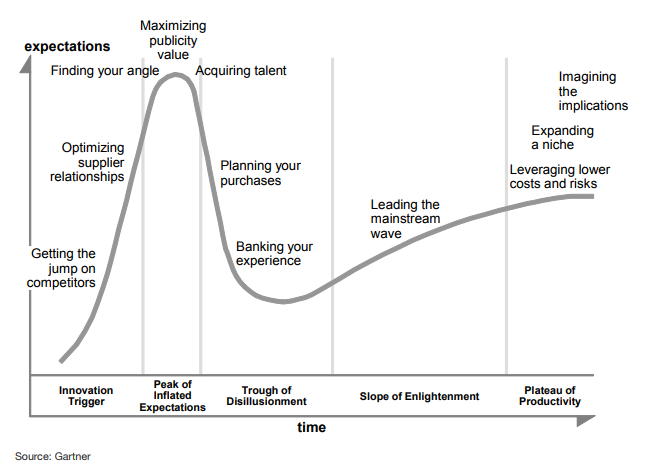
\includegraphics[width=0.8\linewidth,keepaspectratio]{gartner2old}
% \end{center}
% {\tiny (Ref: Understanding Gartner's Hype Cycles - Jackie Fenn, Mark Raskino, Betsy Burton )}
% \end{frame}


% %%%%%%%%%%%%%%%%%%%%%%%%%%%%%%%%%%%%%%%%%%%%%%%%%%%%%%%%%%%%%%%%%%%%%%%%%%%%%%%%%%
% \begin{frame}[fragile]\frametitle{}
% \begin{center}
% {\Large After all this - The Truth \ldots}
% \end{center}
% \end{frame}

% %%%%%%%%%%%%%%%%%%%%%%%%%%%%%%%%%%%%%%%%%%%%%%%%%%%%%%%%%%%
% \begin{frame}[fragile]\frametitle{}
% \begin{center}
% \includegraphics[width=\linewidth,keepaspectratio]{boxquote}
% \end{center}
% \end{frame}



